Na het opstarten van een systeem kan het soms nodig zijn met bestaande processen te stoppen of herstarten omdat er bijvoorbeeld een wijziging in de configuratie is gebeurd, of omdat bepaalde functionaliteit niet langer via deze machine aangeboden wordt. Het kan ook voorkomen dat nieuwe functionaliteit is toegevoegd en dat er een nieuw proces gestart moet worden. Het is dus van belang dat we \texttt{systemd} kunnen vertellen om deze acties uit te voeren. Het commando dat doorvoor beschikbaar is heet \texttt{systemctl}\index{systemctl}. \texttt{systemctl} kent een aantal standaard commando's die we kunnen meegeven. Voor een uitleg van de syntax van het commando verwijzen we naar de man-page. Wij behandelen hier alleen de belangrijkste commando's:
\begin{description}
	\item[start] Start een service
	\item[stop] Stop een service
	\item[restart] Stop een service en als dat klaar is start het weer
	\item[reload] Vraag een service om zijn configuratie opnieuw te laden, kan niet met alle daemons. Dit is niet de Unit-configuratie, maar de configuratie van de daemon zelf.
\end{description}

Om wat ervaring op te doen met \texttt{systemctl} gaan we wat oefenen met een daemon die standaard met de installatie is meegekomen en waar we wat mee kunnen spelen zonder dat het meteen destcructief is voor het systeem. De standaard met de installatie meegekomen daemon is de systemd-timesyncd\index{timesyncd}\index{systemd!timesyncd} daemon. We gaan deze daemon gebruiken om een beetje vertrouwd te raken met \texttt{systemctl}.

\begin{lstlisting}[language=bash]
sudo systemctl status systemd-timesyncd
\end{lstlisting}

\begin{figure}[h]
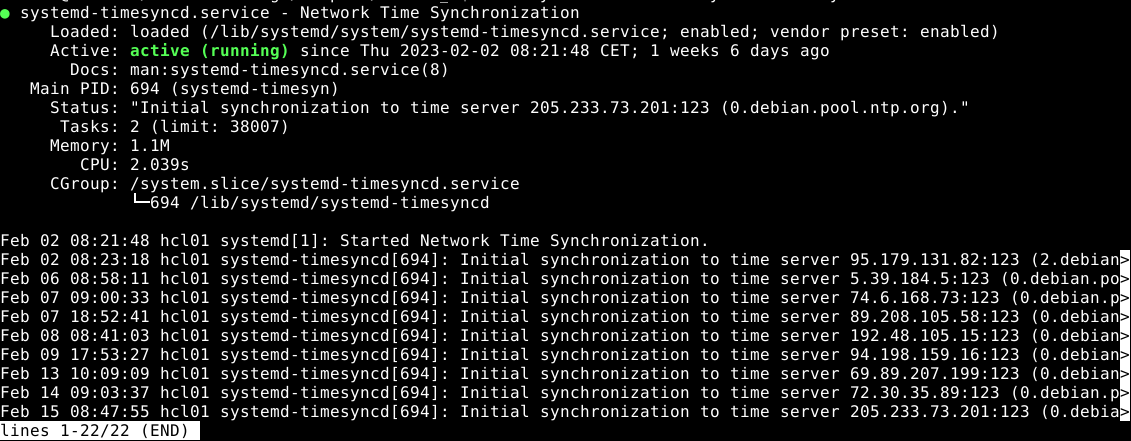
\includegraphics[width=8cm]{systemd-timesyncd-status}
\centering
	\caption{Status output van systemctl}
	\label{scrn:systemd-timesyncd-status}
\end{figure}

Als je net als in het voorbeeld (Figuur \ref{scrn:systemd-timesyncd-status}) een lijn hebt met END dan kan je gebruik maken van 'q' om weer op de command-prompt terecht te komen.

Door aan \texttt{systemctl} de commando's stop of start mee te geven kunnen we daemons op ons systeem stoppen en starten. De tijd synchronisatie daemon is op dit moment gestart, dus het eerste wat we kunnen doen is hem stoppen:

\begin{lstlisting}[language=bash]
sudo systemctl stop systemd-timesyncd
\end{lstlisting}

Met \texttt{systemctl status} kunnen nu de status van de daemon zien en dan zien we dat deze gestopt is. Het opnieuw opstarten doen we met start:

\begin{lstlisting}[language=bash]
sudo systemctl start systemd-timesyncd
\end{lstlisting}

Probeer nu zelf de herstart en reload functies uit. Wat neem je waar?

Om te weten wat \texttt{systemctl} allemaal geladen heeft is er het commando:
\begin{lstlisting}[language=bash]
sudo systemctl list-units
\end{lstlisting}
Hiermee kan je zien wat er allemaal gedaan is door systemd en met \texttt{grep} kan je daar de services uit halen die op dit moment actief zijn:
\begin{lstlisting}[language=bash]
sudo systemctl list-units | grep \.service.*running
\end{lstlisting}

